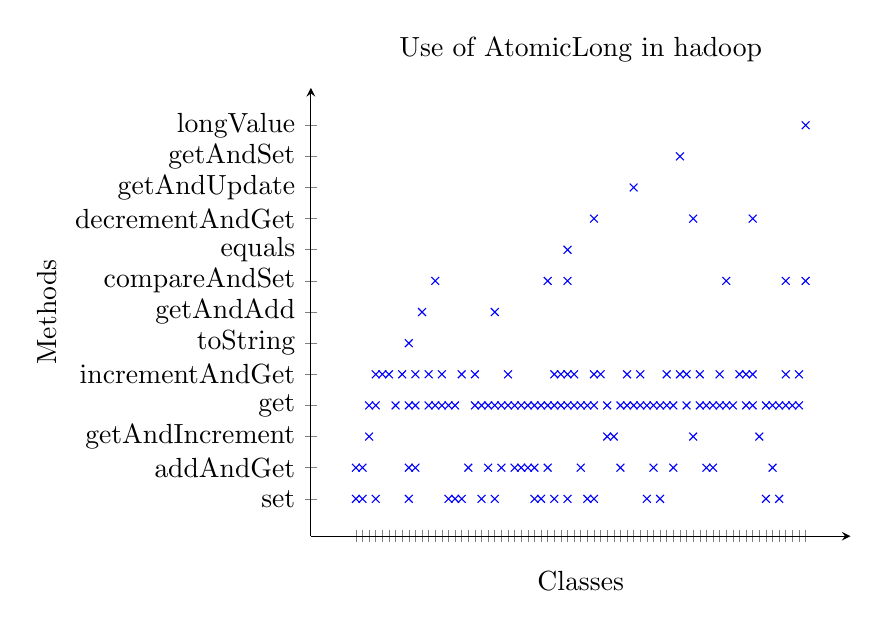
\begin{tikzpicture}
\begin{axis}[scatter/classes={U={mark=+,red}, NU={mark=x,blue}}, legend pos=outer north east,axis x line=bottom, axis y line=left, enlarge x limits=true, xlabel = {Classes}, ylabel = {Methods}, enlarge y limits=true, xtick = data, xticklabels = {,,},ytick=data, yticklabels={set,addAndGet,getAndIncrement,get,incrementAndGet,toString,getAndAdd,compareAndSet,equals,decrementAndGet,getAndUpdate,getAndSet,longValue}, title={Use of AtomicLong in hadoop}]
\addplot[scatter,only marks, scatter src=explicit symbolic]
coordinates {
(0,0) [NU]
(0,1) [NU]
(1,0) [NU]
(1,1) [NU]
(2,2) [NU]
(2,3) [NU]
(3,4) [NU]
(3,0) [NU]
(3,3) [NU]
(4,4) [NU]
(5,4) [NU]
(6,3) [NU]
(7,4) [NU]
(8,0) [NU]
(8,3) [NU]
(8,1) [NU]
(8,5) [NU]
(9,4) [NU]
(9,3) [NU]
(9,1) [NU]
(10,6) [NU]
(11,4) [NU]
(11,3) [NU]
(12,7) [NU]
(12,3) [NU]
(13,4) [NU]
(13,3) [NU]
(14,0) [NU]
(14,3) [NU]
(15,0) [NU]
(15,3) [NU]
(16,4) [NU]
(16,0) [NU]
(17,1) [NU]
(18,4) [NU]
(18,3) [NU]
(19,0) [NU]
(19,3) [NU]
(20,3) [NU]
(20,1) [NU]
(21,0) [NU]
(21,3) [NU]
(21,6) [NU]
(22,3) [NU]
(22,1) [NU]
(23,4) [NU]
(23,3) [NU]
(24,3) [NU]
(24,1) [NU]
(25,3) [NU]
(25,1) [NU]
(26,3) [NU]
(26,1) [NU]
(27,0) [NU]
(27,3) [NU]
(27,1) [NU]
(28,0) [NU]
(28,3) [NU]
(29,7) [NU]
(29,3) [NU]
(29,1) [NU]
(30,4) [NU]
(30,0) [NU]
(30,3) [NU]
(31,4) [NU]
(31,3) [NU]
(32,4) [NU]
(32,0) [NU]
(32,7) [NU]
(32,8) [NU]
(32,3) [NU]
(33,4) [NU]
(33,3) [NU]
(34,3) [NU]
(34,1) [NU]
(35,0) [NU]
(35,3) [NU]
(36,4) [NU]
(36,0) [NU]
(36,3) [NU]
(36,9) [NU]
(37,4) [NU]
(38,2) [NU]
(38,3) [NU]
(39,2) [NU]
(40,3) [NU]
(40,1) [NU]
(41,4) [NU]
(41,3) [NU]
(42,3) [NU]
(42,10) [NU]
(43,4) [NU]
(43,3) [NU]
(44,0) [NU]
(44,3) [NU]
(45,3) [NU]
(45,1) [NU]
(46,0) [NU]
(46,3) [NU]
(47,4) [NU]
(47,3) [NU]
(48,3) [NU]
(48,1) [NU]
(49,4) [NU]
(49,11) [NU]
(50,4) [NU]
(50,3) [NU]
(51,2) [NU]
(51,9) [NU]
(52,4) [NU]
(52,3) [NU]
(53,3) [NU]
(53,1) [NU]
(54,3) [NU]
(54,1) [NU]
(55,4) [NU]
(55,3) [NU]
(56,7) [NU]
(56,3) [NU]
(57,3) [NU]
(58,4) [NU]
(59,4) [NU]
(59,3) [NU]
(60,4) [NU]
(60,3) [NU]
(60,9) [NU]
(61,2) [NU]
(62,0) [NU]
(62,3) [NU]
(63,3) [NU]
(63,1) [NU]
(64,0) [NU]
(64,3) [NU]
(65,4) [NU]
(65,7) [NU]
(65,3) [NU]
(66,3) [NU]
(67,4) [NU]
(67,3) [NU]
(68,7) [NU]
(68,12) [NU]
};
\end{axis}
\end{tikzpicture}